\documentclass{article}
\usepackage[UTF8]{ctex}
\usepackage{geometry}
\usepackage{natbib}
\geometry{left=3.18cm,right=3.18cm,top=2.54cm,bottom=2.54cm}
\usepackage{graphicx}
\usepackage{listings}
\pagestyle{plain}	
\usepackage{setspace}
\usepackage{CJK}
\usepackage{amsmath}
\usepackage{caption2}
\usepackage{datetime} %日期
\renewcommand{\today}{\number\year 年 \number\month 月 \number\day 日}
\renewcommand{\captionlabelfont}{\small}
\renewcommand{\captionfont}{\small}
\usepackage[colorlinks,linkcolor=black]{hyperref}
\begin{document}

\begin{figure}
    \centering
    
\includegraphics[width=8cm]{upc.png}

    \label{figupc}
\end{figure}

	\begin{center}
		\quad \\
		\quad \\
		\heiti \fontsize{45}{17} \quad \quad \quad 
		\vskip 1.5cm
		\heiti \zihao{2} 《信息技术前沿讲座》课程总结报告
		\par 
		循环神经网络
		\par
		Recurrent Neural Network
	\end{center}
	\vskip 1cm
		
	\begin{quotation}
% 	\begin{center}
		\doublespacing
		
        \zihao{4}\par\setlength\parindent{7em}
		\quad 

		学生姓名:\underline{\qquad  吴树晖 \qquad \qquad}

		学\hspace{0.61cm} 号:\underline{\qquad 1808010217\qquad}
		
		专业班级:\underline{\qquad 计算1802 \qquad  }
		
        学\hspace{0.61cm} 院:\underline{计算机科学与技术学院}
% 	\end{center}
		\vskip 1cm
		\centering
		\begin{table}[h]
            \centering 
            \zihao{4}
            \begin{tabular}{|c|c|c|c|c|c|}
            % 这里的rl 与表格对应可以看到,姓名是r,右对齐的;学号是l,左对齐的;若想居中,使用c关键字。
                \hline
                课程认识 & 问题思 考 & 格式规范  & Latex文档制作   & 总分 & 评阅教师 \\
                30\% & 30\% & 20\% & 20\%  &  &  \\
                \hline
                 & & & &  &\\
                & & & &  &\\
                \hline
            \end{tabular}
        \end{table}
		\vskip 2cm
		\today
	\end{quotation}

\thispagestyle{empty}
\newpage
\setcounter{page}{1}
% 在这之前是封面,在这之后是正文
\section{引言}
在前馈神经网络中,信息的传递是单向的,这种限制虽然使得网络变得更容易学习,但在一定程度上也减弱了神经网络模型的能力。在生物神经网络中,神经元之间的连接关系要复杂的多。前馈神经网络可以看着是一个复杂的函数,每次输入都是独立的,即网络的输出只依赖于当前的输入。但是在很多现实任务中,网络的输入不仅和当前时刻的输入相关,也和其过去一段时间的输出相关。比如一个有限状态自动机,其下一个时刻的状态(输出)不仅仅和当前输入相关,也和当前状态(上一个时刻的输出)相关,这种模型我们一般称为时序模型。时间序列可以抽象的表示为一个向量序列:
$$x_1,x_2,x_3,...,x_n$$
其中,$x_i$是向量,下标$i$为时刻。各个时刻之间的向量之间存在相关。算法需要根据输入的序列来产生输出值。这类问题称为序列预测问题。
\par 
语音识别和自然语言处理是序列预测问题的典型代表,前者的输入时一个语音信号序列,后者是一个文字序列。
神经网络每次的输入为一个词(实际上是对这个词进行编码后的向量),最后要填出这个空,这需要神经网络能够理解语义,并记住之前输入的信息,即语句上下文。前馈网络是一个静态网络,明显不能不处理这种情况。此外,序列数据的长度一般是不固定的,比如视频、语音、文本等。而前馈神经网络要求输入和输出的维数都是固定的,不能任意改变。因此,当处理这一类和时序相关的问题时,就需要一种能力更强的模型。\par 
循环神经网络循环神经网络(Recurrent NeuralNetworks,RNN)通过使用带自反馈的神经元,能够处理任意长度的序列。RNN也经常被翻译为递归神经网络。这里为了区别与另外一种递归神经网络(RecursiveNeural Networks),我们称为循环神经网络。

\section{RNN的网络结构}
循环神经网络由输入层、循环层和输出层构成,可能还包括全连接神经网络中的全连层。输入层和输出层与前馈型神经网络类似,唯一不同的是循环层。
下图是一个简单的循环神经网络:\par 
\centerline{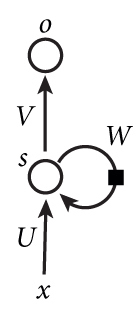
\includegraphics[height=6cm]{0}}
在上图中,$x$是一个向量,它表示输入层的值(这里面没有画出来表示神经元节点的圆圈);$s$是一个向量,它表示隐藏层的值(这里隐藏层面画了一个节点,你也可以想象这一层其实是多个节点,节点数与向量$s$的维度相同);$U$是输入层到隐藏层的权重矩阵,$o$也是一个向量,它表示输出层的值;$V$是隐藏层到输出层的权重矩阵。循环神经网络的隐藏层的值$s$不仅仅取决于当前这次的输入$x$,还取决于上一次隐藏层的值$s$。权重矩阵$W$就是隐藏层上一次的值作为这一次的输入的权重。
\par 
我们要对循环层和输出层进行重点分析。
\subsection{循环层}
循环神经网络具有记忆功能,它会记住网络在上一时刻运行时产生的状态值,并将该值用于当前时刻输出值的生成。
我们把RNN简单结构图的图展开,循环神经网络也可以画成下面这个样子:\par
\centerline{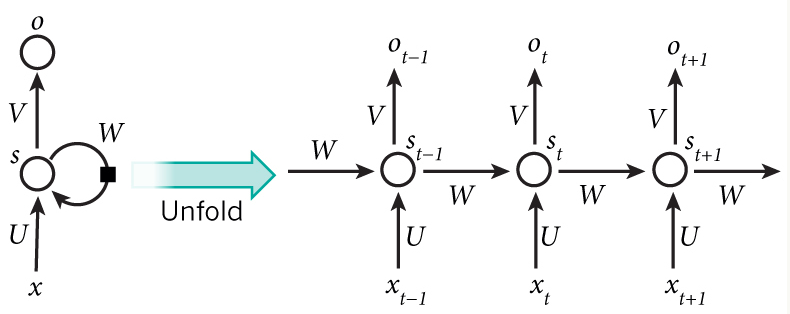
\includegraphics[width=13cm]{2}}
\par 
上图这个网络在t时刻接收到输入$x_t$之后网络会产生一个输出$y_t$,而这个输出是由之前时刻的输入序列共同决定的。假设$t$时刻的状态值为$h_t$,它由上一时刻的状态值$h_{t-1}$,以及当前时刻的输入值$x_t$,共同决定的,即:
$$h_t=f(h_{t-1},x_t)$$
这是一个递推的定义,现在的问题是如何确定这个递推公式。假设$t$时刻循环层的输人向量为$x_t$,输出向量为$h_t$,上一时刻的输出值为$h_{t-1}$,$f$为激活函数,则循环层输出的状态值的计算公式为:
$$h_t= f(W_{xh}x_t+W_{hh}h_{t-1}+b)$$
其中,$W_{xh}$为输入层到隐含层的权重矩阵;$W_{hh}$为隐含层内的权重矩阵,可以看作状态转移权重;$b$为偏置向量bias。从上面的计算公式可以看出,循环层任意一个神经元的当前时刻状态值与该循环层所有神经元在上一时刻的状态值、当前时刻输入向量的任何一个分量都有关系。与前馈型神经网络相比,这里多了一个项$W_{hh}h_{t-1}$它意味着使用了隐含层上次的输出值。我们选用tanh作为激活函数,这样隐含层的变换为
$$h_t= tanh(W_{xh}x_t+W_{hh}h_{t-1}+b)$$
使用tanh的原因是为了保证神经网络的映射函数是非线性的。\par 
在这里$h_{t-1}$和$x_t$共同决定$h_t$,$h_{t-1}$体现了记忆功能,而它
的值又由里$h_{t-2}$和$x_{t-1}$决定。依次展开之后,$h_t$的值实际上是由$x_1,x_2,x_3,…,x_t$决定的,它记住了之前完整的序列信息。权重矩阵$W_{hh}$并不会随着时间变化,在每个时刻进行计算时使用的是同一个矩阵。这样做的好处是,一方面是减少了模型参数,另一方面也记住了之前的信息。\par 

\subsection{输出层}
输出层以循环层的输出值作为输入并产生循环神经网络最终的输出,它不具有记忆功能,输出层实现的变换为:
$$y_t=g(W_0h_t+b_0)$$
其中,$W_0$为权重矩阵,$b_0$为偏置向量,$g$为变换函数。变换函数的类型根据任务而定,对于分类任务一般选用$softmax$函数,输出各个类的概率。在这里只使用了一个循环层,实际使用时可以有多个循环层,


\subsection{深层网络}
上面介绍的循环神经网络只有一个输入层、一个循环层和一个输出层。与全连接神经网络以及卷积神经网络一样,可以把它推广到任意多个隐含层的情况,得到深层循环神经网络。\par 
这里有3种方案:\par 
第一种方案称为 Deep\quad Input-to-Hidden\quad Function,它在循环层之前加入多个普通的全连接层,将输入向量进行多层映射之后再送入循环层进行处理。\par
第二种方案是Deep\quad Hidden-to-Hidden\quad Transition,它使用多个循环层,这与前馈型神经网络类似,唯一不同的是计算隐含层输出的时候需要利用本隐含层上一时刻的值。\par 
第三种方案是 Deep\quad Hidden-to-Output\quad Function,它在循环层到输出层之间加入多个全连接层,这与第一种情况类似。\par 
由于循环层一般用tanh作为激活函数,层次过多之后会导致梯度消失问题,可以采用跨层连接的方案。

\section{RNN网络的训练}
我们可以采用Back\quad Propagation\quad Through\quad Time(BPTT)算法
\par
循环神经网络的每个训练样本是一个时间序列,同一个训练样本前后时刻的输入值之间有关联,每个样本的序列长度可能不相同。训练时先对这个序列中每个时刻的输入值进行正向传播,再通过反向传播计算出参数的梯度值并更新参数。
\subsection{以简单RNN网络为例}
我们通过有一个输入层,一个循环层和一个输出层的简单RNN网络为例:\par 
\centerline{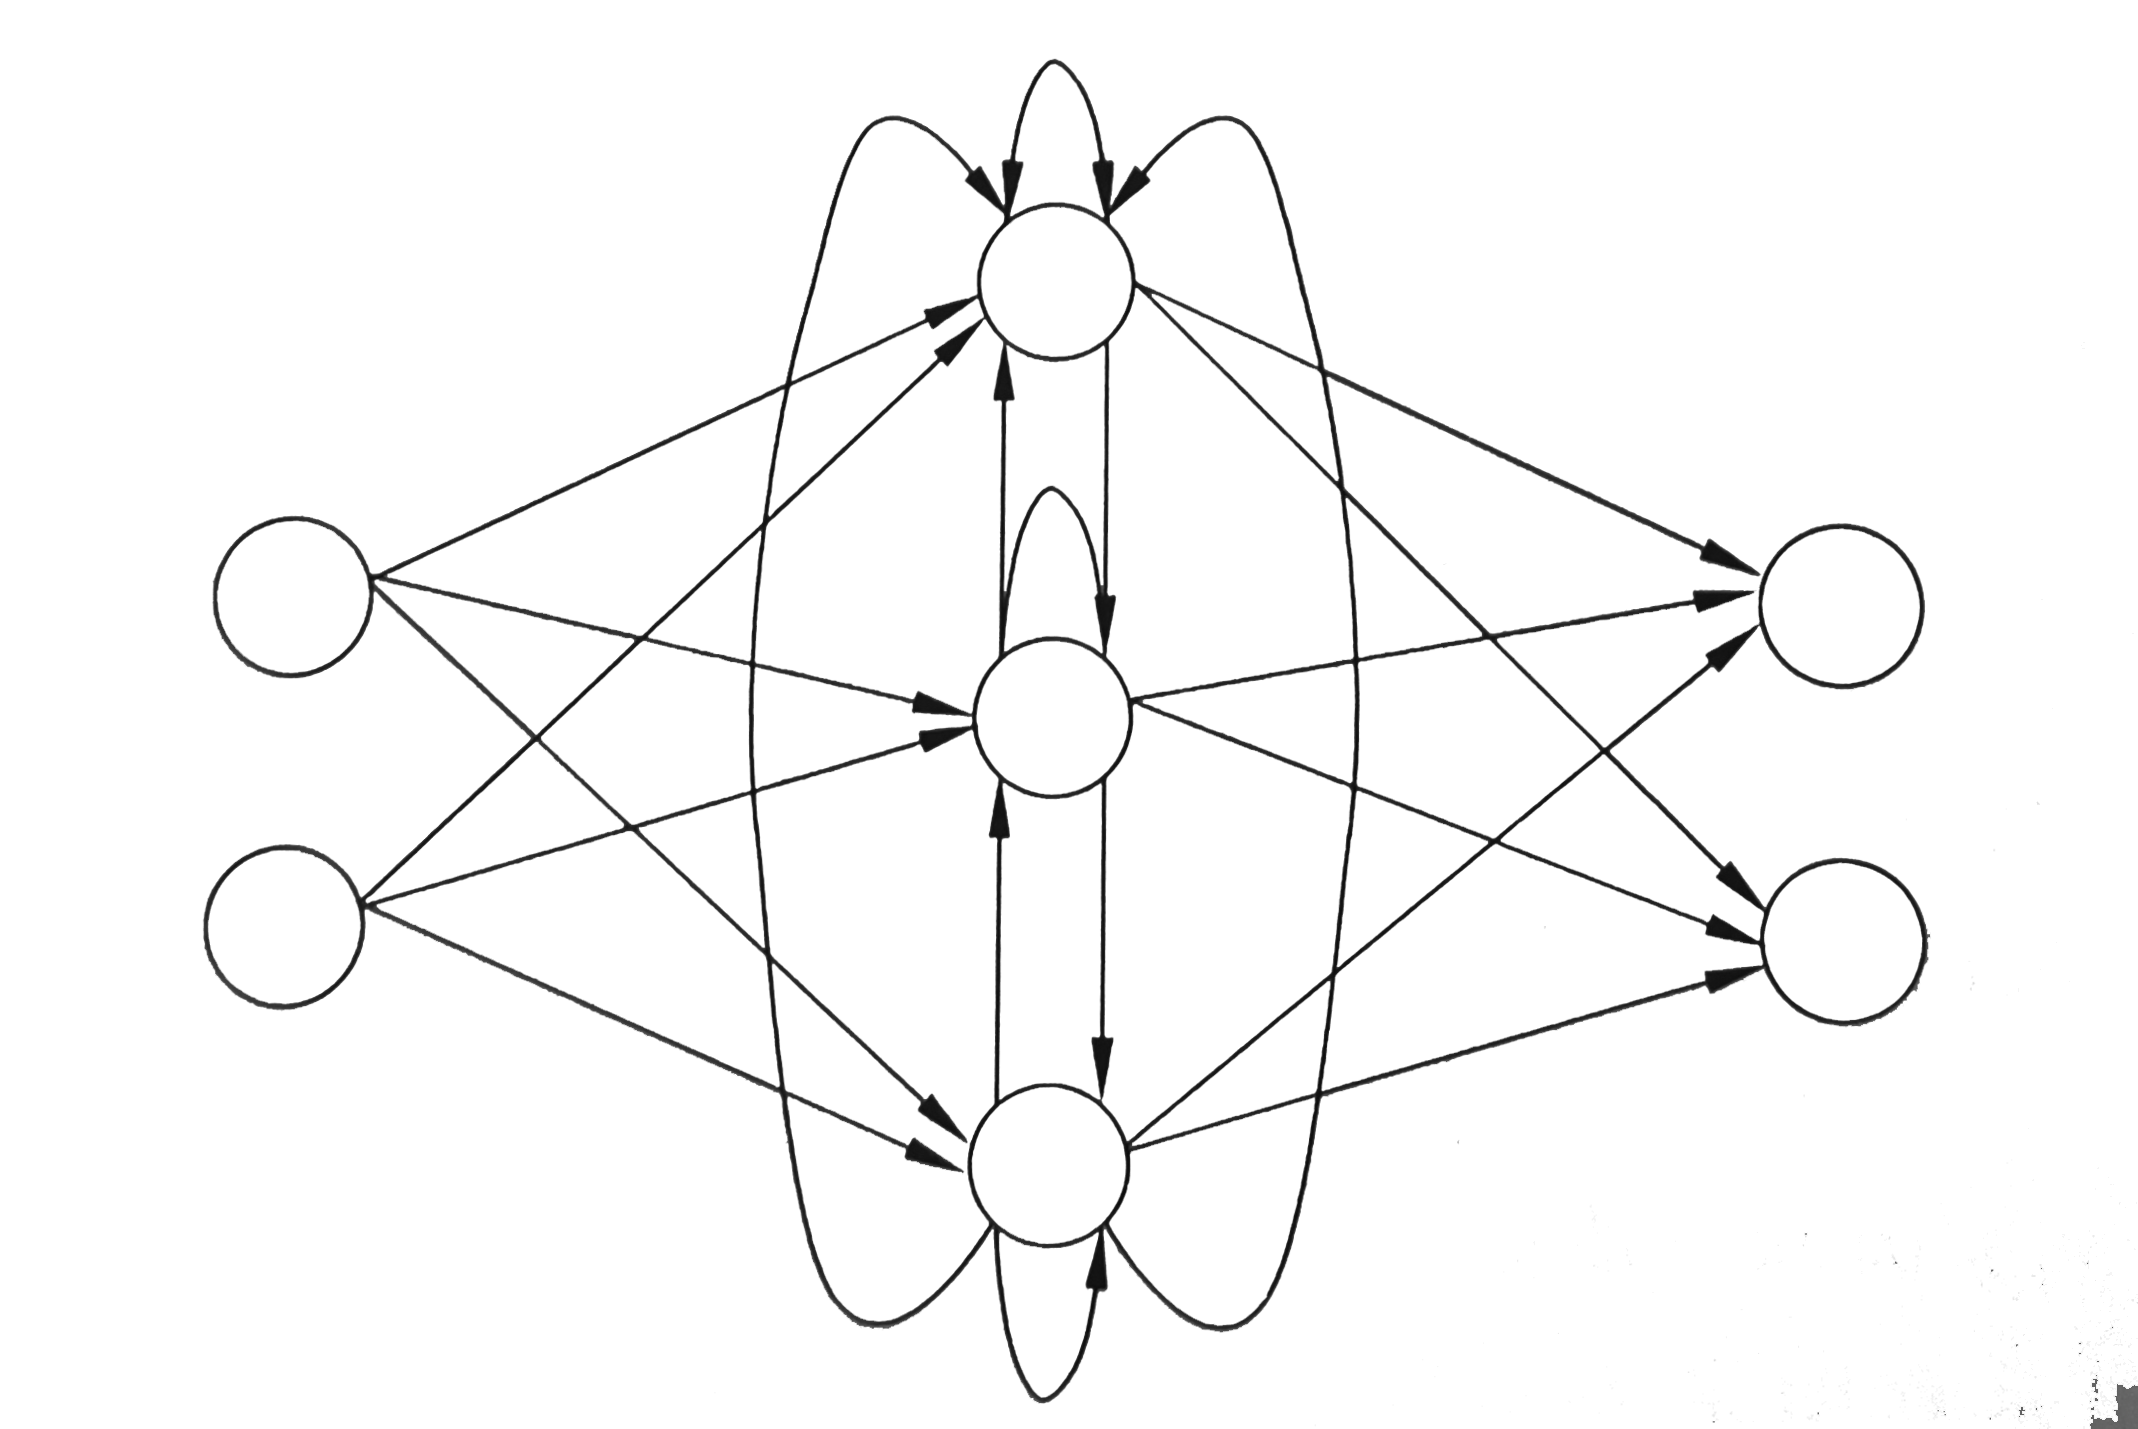
\includegraphics[width=13cm]{mod1}}
网络的输入层有2个神经元,循环层有3个神经元,输出层有2个神经元。\par 
假设有一个训练样本,其序列值为:
$$(x_1,y_1),(x_2,y_2),(x_3,y_3)$$
其中,$x_i$为输入向量,$y_i$为标签向量。循环层状态的初始值设置为0.在$t=1$时刻,网络的输出为
$$u_1=W_{xh}x_1+b_h$$
$$h_1=f(u_1)$$
$$v_1=W_0h_1+b_0$$
$$y_1^*=g(v_1)$$
在$t=2$时刻,网络的输出为
$$u_2=W_{xh}x_2+W_{hh}f(W_{xh}x_1+b_h)+b_h$$
$$h_2=f(u_2)$$
$$v_2=W_0h_2+b_0$$
$$y_2^*=g(v_2)$$
在$t=3$时刻,网络的输出为
$$u_3=W_{xh}x_3+W_{hh}f(W_{xh}x_2+W_{hh}f(W_{xh}x_1+b_h)+b_h)+b_h$$
$$h_3=f(u_3)$$
$$v_3=W_0h_3+b_0$$
$$y_3^*=g(v_3)$$
对单个样本的序列数据,定义t时刻的损失函数为
$$L_t=L(y_t,y_t^*)$$
总损失函数为各个时刻损失函数之和
$$L=\sum_{t=1}^{3}L(y_t,y_t^*)$$
如果输出层使用softmax变换,损失函数使用交叉熵,则有
$$L_t=-y^T_tln(y_t^*)$$
可以得到梯度的计算公式
$$\nabla _{v_t}{L_t}=y_t^*-y_t$$
在t时刻损失函数对输出层权重的梯度为
$$\nabla _{w_0}{L_t}=(\nabla _{v_t}{L_t})h_t^T=(y_t^*-y_t)h_t^T$$
对偏置项的梯度为
$$\nabla _{b_0}{L_t}=\nabla _{v_t}{L_t}=y_t^*-y_t$$
总损失函数对权重的梯度为
$$\nabla _{w_0}{L_t}=\sum_{t=1}^{3}((y_t^*-y_t)h_t^T)$$
对偏置项的梯度为
$$\nabla _{b_0}{L_t}=\sum_{t=1}^{3}(y_t^*-y_t)$$
下面来看隐含层,与输出层相比情况更复杂。按时间展开之后,各个时刻隐含层的输出值是权重矩阵和偏置向量的复合函数,与全连接神经网络类似,但这种复合是在时间轴上的,每次都用同一个权重矩阵。全连接神经网络是在各个神经元层之间进行的,各个层的重权矩阵不同。 
\par
在$t=1$时刻,$W_{xh}$的梯度为
$$
\nabla _{w_{xh}}{L_1} =(\nabla_{u_1}L_1)x_1^T=((\nabla_{h_1}L_1)\odot f^{'}(u_1))x_1^T=((W_0^T(\nabla_{v_1}L_1))\odot f^{'}(u_1))x_1^T
$$
$$
\nabla _{w_{xh}}{L_1} =((W_0^T(y_1^*=y_1))\odot f^{'}(u_1))x_1^T
$$
由于$t=1$时刻隐含层的输出值与$W$无关,因此
$$\nabla _{w_{hh}}{L_1} = 0$$
对偏置项
$$\nabla _{b_h}{L_1}=\nabla _{u_1}{L_1}=(W_0^T(y_1^*=y_1))\odot f^{'}(u_1)$$
在$t=2$时刻,因为
$$u_2=W_{xh}x_2+W_{hh}f(W_{xh}x_1+b_h)+b_h$$
在公式中$W_{xh}$出现了两次,此时损失函数对权重$W_{xh}$的梯度为
$$\nabla _{w_{xh}}{L_2}=(\nabla _{u_2}L_2)x_2^T+(\nabla_{u_1}L_2)x_1^T$$
由于
$$u_2=W_{xh}x_2+W_{hh}f(u_1)+b_h$$
易得
$$\nabla_{u_1}L_2=\nabla _{h_1}L_2\odot f^{'}(u_1)=W^T_{hh}(\nabla _{u_2}L_2)\odot f^{'}(u_1)$$
代入上式可以得到
$$\nabla _{w_{xh}}{L_2}=((W_0^T(\nabla _{v_2}L_2))\odot f^{'}(u_2) )x_2^T+(W_{hh}^T((W^T_{0}(\nabla _{v_2}L_2)\odot f^{'}(u_2))\odot f^{'}(u_1))x_1^T$$
计算$\nabla W_{hh}L_2$
$$\nabla W_{hh}L_2=(\nabla _{u_2}L_2)h_1^T=((\nabla _{h_2}L_2)\odot  f^{'}(u_2))h_1^T$$
$$\nabla W_{hh}L_2=((W_0^T(\nabla _{v_2}L_2))\odot f^{'}(u_2))h_1^T$$
在$t=3$时刻,与$t=2$时刻类似,我们可以得到
$$u_{3}=W_{xh}x_3+W_{hh}f(W_{xh}x_2+W_{hh}f(u_1)+b_h)+b_h$$
$$\nabla _{w_{xh}}{L_3}=(\nabla _{u_3}L_3)x_3^T+(\nabla _{u_2}L_3)x_2^T+(\nabla_{u_1}L_3)x_1^T$$
$$\nabla_{u_2}L_3=\nabla _{h_2}L_3\odot f^{'}(u_2)=W^T_{hh}(\nabla _{u_3}L_3)\odot f^{'}(u_2)$$
$$\nabla_{u_1}L_3=\nabla _{h_1}L_3\odot f^{'}(u_1)=W^T_{hh}(\nabla _{u_2}L_3)\odot f^{'}(u_1)$$
可以得到$\nabla W_{xh}L_3$。类似可以计算出$\nabla W_{hh}L_3$,我们可以得到总损失函数对各个参数的偏导数:
$$\nabla W_{xh}L = \sum_{t=1}^{3}\nabla W_{xh}L_t$$
$$\nabla W_{hh}L = \sum_{t=1}^{3}\nabla W_{hh}L_t$$
然后我们可以使用梯度下降法(或牛顿法、拟牛顿法等机器学习方法)进行参数更新。(参数更新方法可以参考计科1804杨世骄报告)
\section{应用举例}
\subsection{基于RNN的语言模型}
我们首先把词依次输入到循环神经网络中,每输入一个词,循环神经网络就输出截止到目前为止,下一个最可能的词。例如,当我们依次输入:
\begin{lstlisting}[ frame=shadowbox]
	我 昨天 上学 迟到 了
\end{lstlisting}
神经网络的输出如下图所示:\par
\centerline{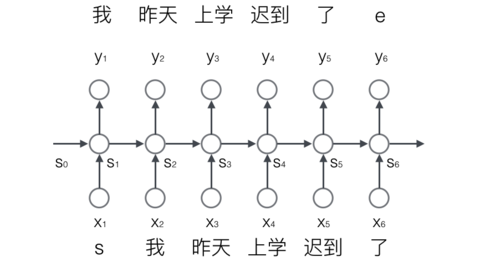
\includegraphics[width=12cm]{language}}
其中,s和e是两个特殊的词,分别表示一个序列的开始(Start)和结束(End)。
\subsection{机器翻译}
机器翻译类似于语言建模,因为我们的输入是源语言(例如德语)中的单词序列。我们希望用我们的目标语言(例如英语)输出一系列单词。关键区别是,我们的输出只有在看到完整输入后才开始,因为我们翻译句子的第一个单词可能需要从完整的输入序列中捕获的信息。\par 
\centerline{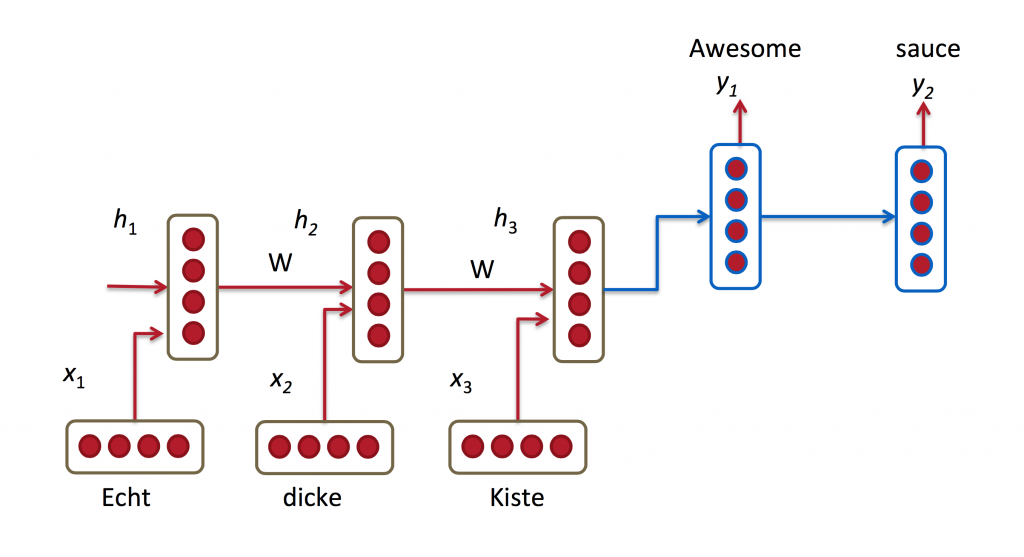
\includegraphics[width=12cm]{tran}}
相关论文:\par 
\href{https://www.aclweb.org/anthology/P14-1140.pdf}{A Recursive Recurrent Neural Network
	for Statistical Machine Translation}\par
\href{http://papers.nips.cc/paper/5346-sequence-to-sequence-learning-with-neural-networks.pdf}{Sequence to Sequence Learning with Neural Networks}\par
\href{https://www.microsoft.com/en-us/research/wp-content/uploads/2016/02/EMNLP2013RNNMT.pdf}{Joint Language and Translation Modeling with Recurrent Neural Networks}\par
\subsection{语音识别}
给定声波的声学信号输入序列,我们可以预测一系列语音段及其概率。\par
相关论文:\par 
\href{http://proceedings.mlr.press/v32/graves14.pdf}{Towards End-to-End Speech Recognition
with Recurrent Neural Networks}
\subsection{生成图像描述}
根据图像生成相对应的描述文字(看图说话)。\par 
\centerline{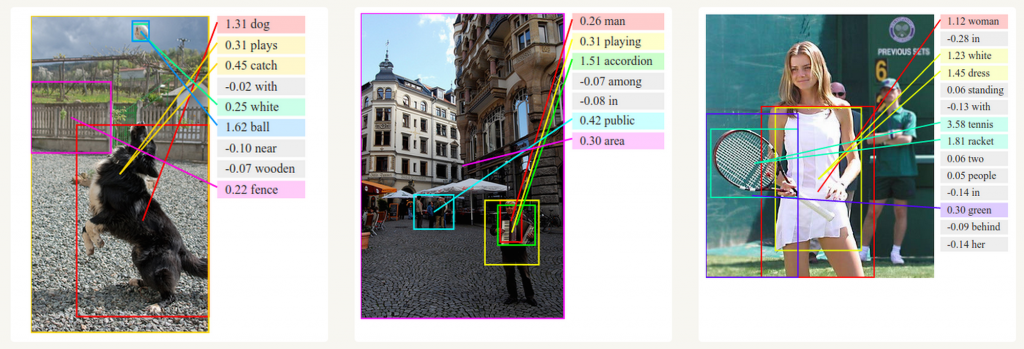
\includegraphics[width=12cm]{GID}}


\section{RNN的挑战及改进措施}
\subsection{梯度爆炸和梯度消失}
RNN在训练中很容易发生梯度爆炸和梯度消失,这导致训练时梯度不能在较长序列中一直传递下去,从而使RNN无法捕捉到长距离的影响。我们给出误差项沿时间反向传播的算法。\par 
\centerline{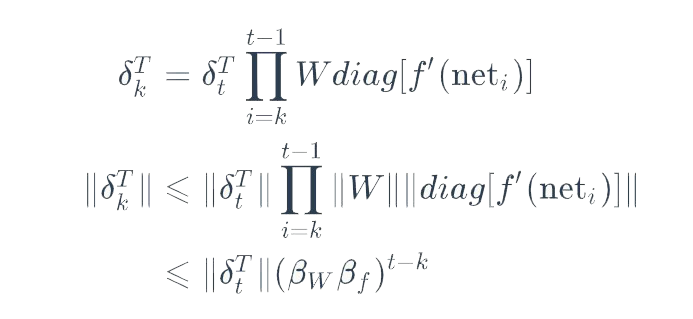
\includegraphics[width=8cm]{10}}
上式的$\beta$定义为矩阵的模的上界。因为上式是一个指数函数,如果t-k很大的话(也就是向前看很远的时候),会导致对应的误差项的值增长或缩小的非常快,这样就会导致相应的梯度爆炸和梯度消失问题(取决于$\beta$大于1还是小于1)。\par 
通常来说,梯度爆炸更容易处理一些。因为梯度爆炸的时候,我们的程序会收到NaN错误。我们也可以设置一个梯度阈值,当梯度超过这个阈值的时候可以直接截取。
\par 
梯度消失更难检测,而且也更难处理一些。总的来说,我们有三种方法应对梯度消失问题:
\begin{itemize}
	\item 合理的初始化权重值。初始化权重,使每个神经元尽可能不要取极大或极小值,以躲开梯度消失的区域。
	\item 使用relu代替sigmoid和tanh作为激活函数。原理请参考上一篇文章零基础入门深度学习(4) - 卷积神经网络的激活函数一节。
	\item 使用其他结构的RNNs,比如长短时记忆网络(LTSM)和Gated Recurrent Unit(GRU),这是最流行的做法。
\end{itemize}
 
\subsection{长短期记忆模型}
长短期记忆模型(Long short-term memory, LSTM)是一种特殊的RNN,主要是为了解决长序列训练过程中的梯度消失和梯度爆炸问题。简单来说,就是相比普通的RNN,LSTM能够在更长的序列中有更好的表现。\par 
LSTM结构(图右)和普通RNN的主要输入输出区别如下所示。\par 
\centerline{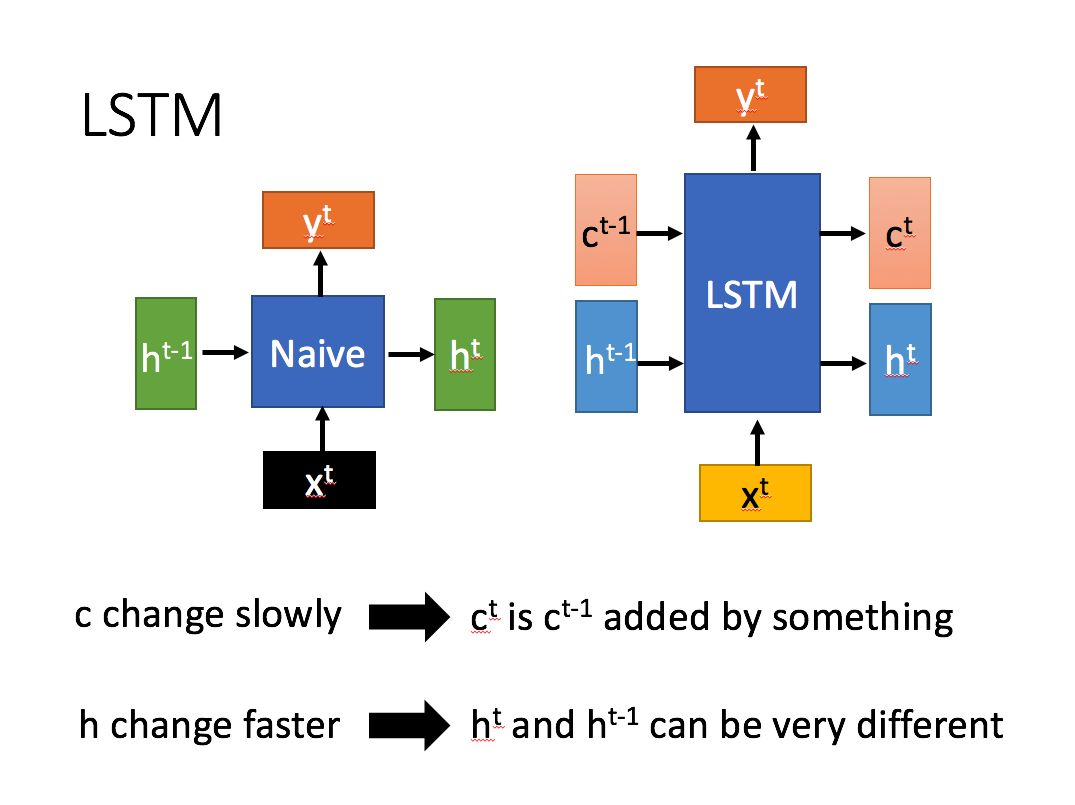
\includegraphics[width=10cm]{lstmi}}
LSTM的内部结构通过三个门控状态来控制传输状态,记住需要长时间记忆的,忘记不重要的信息;这点与RNN的记忆叠加方式不同。对很多需要“长期记忆”的任务来说,尤其好用。\par 
但也因为引入了很多内容,导致参数变多,也使得训练难度加大了很多。
\subsection{门控循环模型}
门控循环模型(Gate Recurrent Unit,GRU)是循环神经网络(Recurrent Neural Network, RNN)的一种。和LSTM(Long-Short Term Memory)一样,也是为了解决长期记忆和反向传播中的梯度等问题而提出来的。GRU输入输出的结构与普通的RNN相似,其中的内部思想与LSTM相似。与LSTM相比,GRU内部少了一个”门控“,参数比LSTM少,但是却也能够达到与LSTM相当的功能。考虑到硬件的计算能力和时间成本,因而很多时候会更加倾向于选择GRU。\par
GRU的输入输出结构与普通的RNN是一样的。
\subsection{双向网络}
对于语言模型来说,光看前面的词是不够的,比如下面这句话:
\begin{lstlisting}[ frame=shadowbox]
我的手机坏了,我打算____一部新手机。
\end{lstlisting}
如果我们只看横线前面的词,此处可以填维修、购买、大哭等,这些无法确定,甚至可能出现概率相等。但如果我们也看到了横线后面的词是『一部新手机』,那么,横线上的词填『买』的概率就大得多了。\par 
基本循环神经网络是无法对此进行建模的,因此,我们需要双向循环神经网络,如下图所示: \par 
\centerline{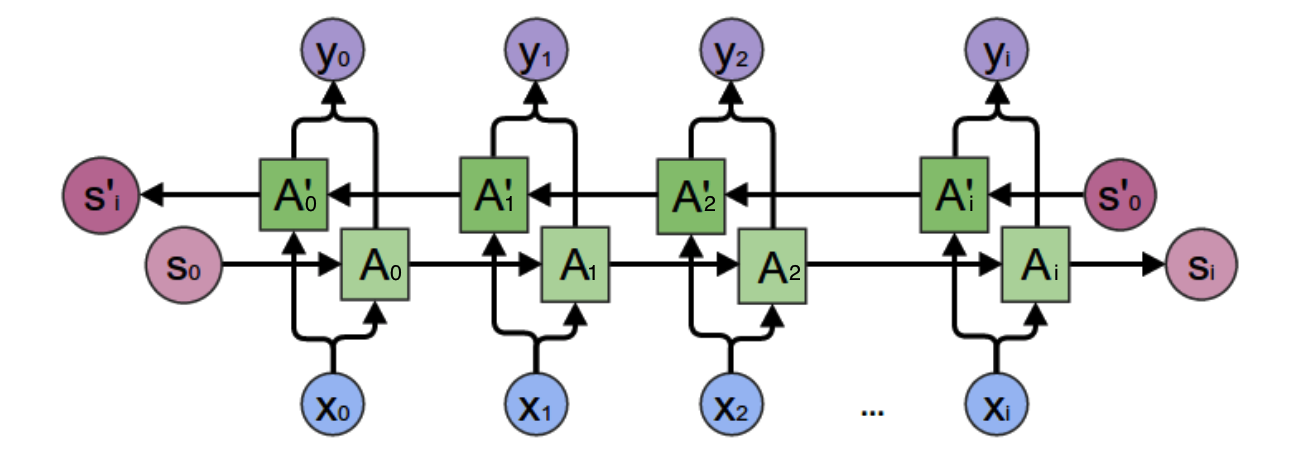
\includegraphics[width=12cm]{shuangxiang}}

\section{总结}
讲座的内容很充实,形式也十分丰富,讲座的主题也涵盖了包括但不限于数据库原理、大数据、人工智能等等前沿知识,在技术之外,我们更多的了解了计算机与实际相结合,无论是产业还是社会政治领域,计算机科学都有很大的发展空间。通过前沿技术讲座课程,我更加坚定了自己的方向-自然语言处理和大数据分析。\par 
人工智能在历史上曾经历三起三落,现在正是人工智能技术走上坡路的时期,随着数据量的不断增长、数据硬件存储能力的扩增以及数据计算能力的提升与计算成本的降低,机器学习算法的实现有了无限可能。\par 
另外,随着理论研究的不断深入,机器学习在传统领域的基础上,又扩展出了多个分支—强化学习、深度学习、多任务学习,等等。应用领域也得以扩展,从数据挖掘、图像检测、模式识别到自然语言处理等等,可以说机器学习已经遍及到人们生活的方方面面。\par
\subsection{人工智能的“三起三落”}
人工智能的第一次高峰:在1956年的这次会议之后,人工智能迎来了属于它的第一段高峰。在这段长达十余年的时间里,计算机被广泛应用于数学和自然语言领域,用来解决代数、几何和英语问题。这让很多研究学者看到了机器向人工智能发展的信心。甚至在当时,有很多学者认为:“二十年内,机器将能完成人能做到的一切。” \par 

人工智能第一次低谷: 70年代,人工智能进入了一段痛苦而艰难岁月。由于科研人员在人工智能的研究中对项目难度预估不足,不仅导致与美国国防高级研究计划署的合作计划失败,还让大家对人工智能的前景蒙上了一层阴影。与此同时,社会舆论的压力也开始慢慢压向人工智能这边,导致很多研究经费被转移到了其他项目上。\par 
在当时,人工智能面临的技术瓶颈主要是三个方面,第一,计算机性能不足,导致早期很多程序无法在人工智能领域得到应用;第二,问题的复杂性,早期人工智能程序主要是解决特定的问题,因为特定的问题对象少,复杂性低,可一旦问题上升维度,程序立马就不堪重负了;第三,数据量严重缺失,在当时不可能找到足够大的数据库来支撑程序进行深度学习,这很容易导致机器无法读取足够量的数据进行智能化。  \par 
人工智能的崛起:1980年,卡内基梅隆大学为数字设备公司设计了一套名为XCON的“专家系统”。这是一种,采用人工智能程序的系统,可以简单的理解为“知识库+推理机”的组合,XCON是一套具有完整专业知识和经验的计算机智能系统。在这个时期,仅专家系统产业的价值就高达5亿美元。 \par 
人工智能第二次低谷:可怜的是,命运的车轮再一次碾过人工智能,让其回到原点。仅仅在维持了7年之后,这个曾经轰动一时的人工智能系统就宣告结束历史进程。到1987年时,苹果和IBM公司生产的台式机性能都超过了Symbolics等厂商生产的通用计算机。从此,专家系统风光不再。 \par 
人工智能再次崛起:上世纪九十年代中期开始,随着AI技术尤其是神经网络技术的逐步发展,以及人们对AI开始抱有客观理性的认知,人工智能技术开始进入平稳发展时期。1997年5月11日,IBM的计算机系统“深蓝”战胜了国际象棋世界冠军卡斯帕罗夫,又一次在公众领域引发了现象级的AI话题讨论。这是人工智能发展的一个重要里程。 2016年,alphago在围棋上击败了李世石,再一次向世人揭示了人工智能非凡力量。
\subsection{自然语言处理的问题}
一是语义理解,或者说知识的学习,或常识的学习问题。这是自然语言处理技术如何变得更“深”的问题。尽管常识的理解对人类来说不是问题,但是它却很难被教给机器。比如我们可以对手机助手说“查找附近的餐馆”,手机就会在地图上显示出附近餐馆的位置。但你如果说“我饿了”,手机助手可能就无动于衷,因为它缺乏“饿了需要就餐”这样的常识,除非手机设计者把这种常识灌入到了这个系统中。但大量的这种常识都潜藏在我们意识的深处,AI系统的设计者几乎不可能把所有这样的常识都总结出来,并灌入到系统中。
\par 
二是低资源问题。所谓无监督学习、Zero-shot学习、Few-shot学习、元学习、迁移学习等技术,本质上都是为了解决低资源问题。面对标注数据资源贫乏的问题,譬如小语种的机器翻译、特定领域对话系统、客服系统、多轮问答系统等,自然语言处理尚无良策。这类问题统称为低资源的自然语言处理问题。对这类问题,我们除了设法引入领域知识(词典、规则)以增强数据能力之外,还可以基于主动学习的方法来增加更多的人工标注数据,以及采用无监督和半监督的方法来利用未标注数据,或者采用多任务学习的方法来使用其他任务,甚至其他语言的信息,还可以使用迁移学习的方法来利用其他的模型。这是自然语言处理技术如何变得更“广”的问题。
\subsection{自然语言处理的发展方向}
微软亚洲研究院副院长、ACL主席周明博士发表署名文章《LP将迎来黄金十年》中指出,NLP将向四个方面倾斜,分别是:\par
1)将知识和常识引入到目前基于数据的学习系统中;\par 
2)低资源的NLP任务的学习方法;\par 
3)上下文建模、多轮语义理解;\par 
4)基于语义分析、知识和常识的可解释NLP。

\section{附录}
\subsection{RNN实现代码}
\href{https://github.com/hellopteromyini/RNN-Based-on-TF/tree/master}{Github}
\subsection{社交平台及博客主页}
\begin{itemize}
	\item 自建博客
	\par
	\url{https://upcwsh.top}
	\par
	\centerline{
\includegraphics[width=12cm]{myblog}}
	\centerline{自建博客}	
	\par 
    \item Github主页
    \par
    \url{https://github.com/hellopteromyini}
    \par
	\centerline{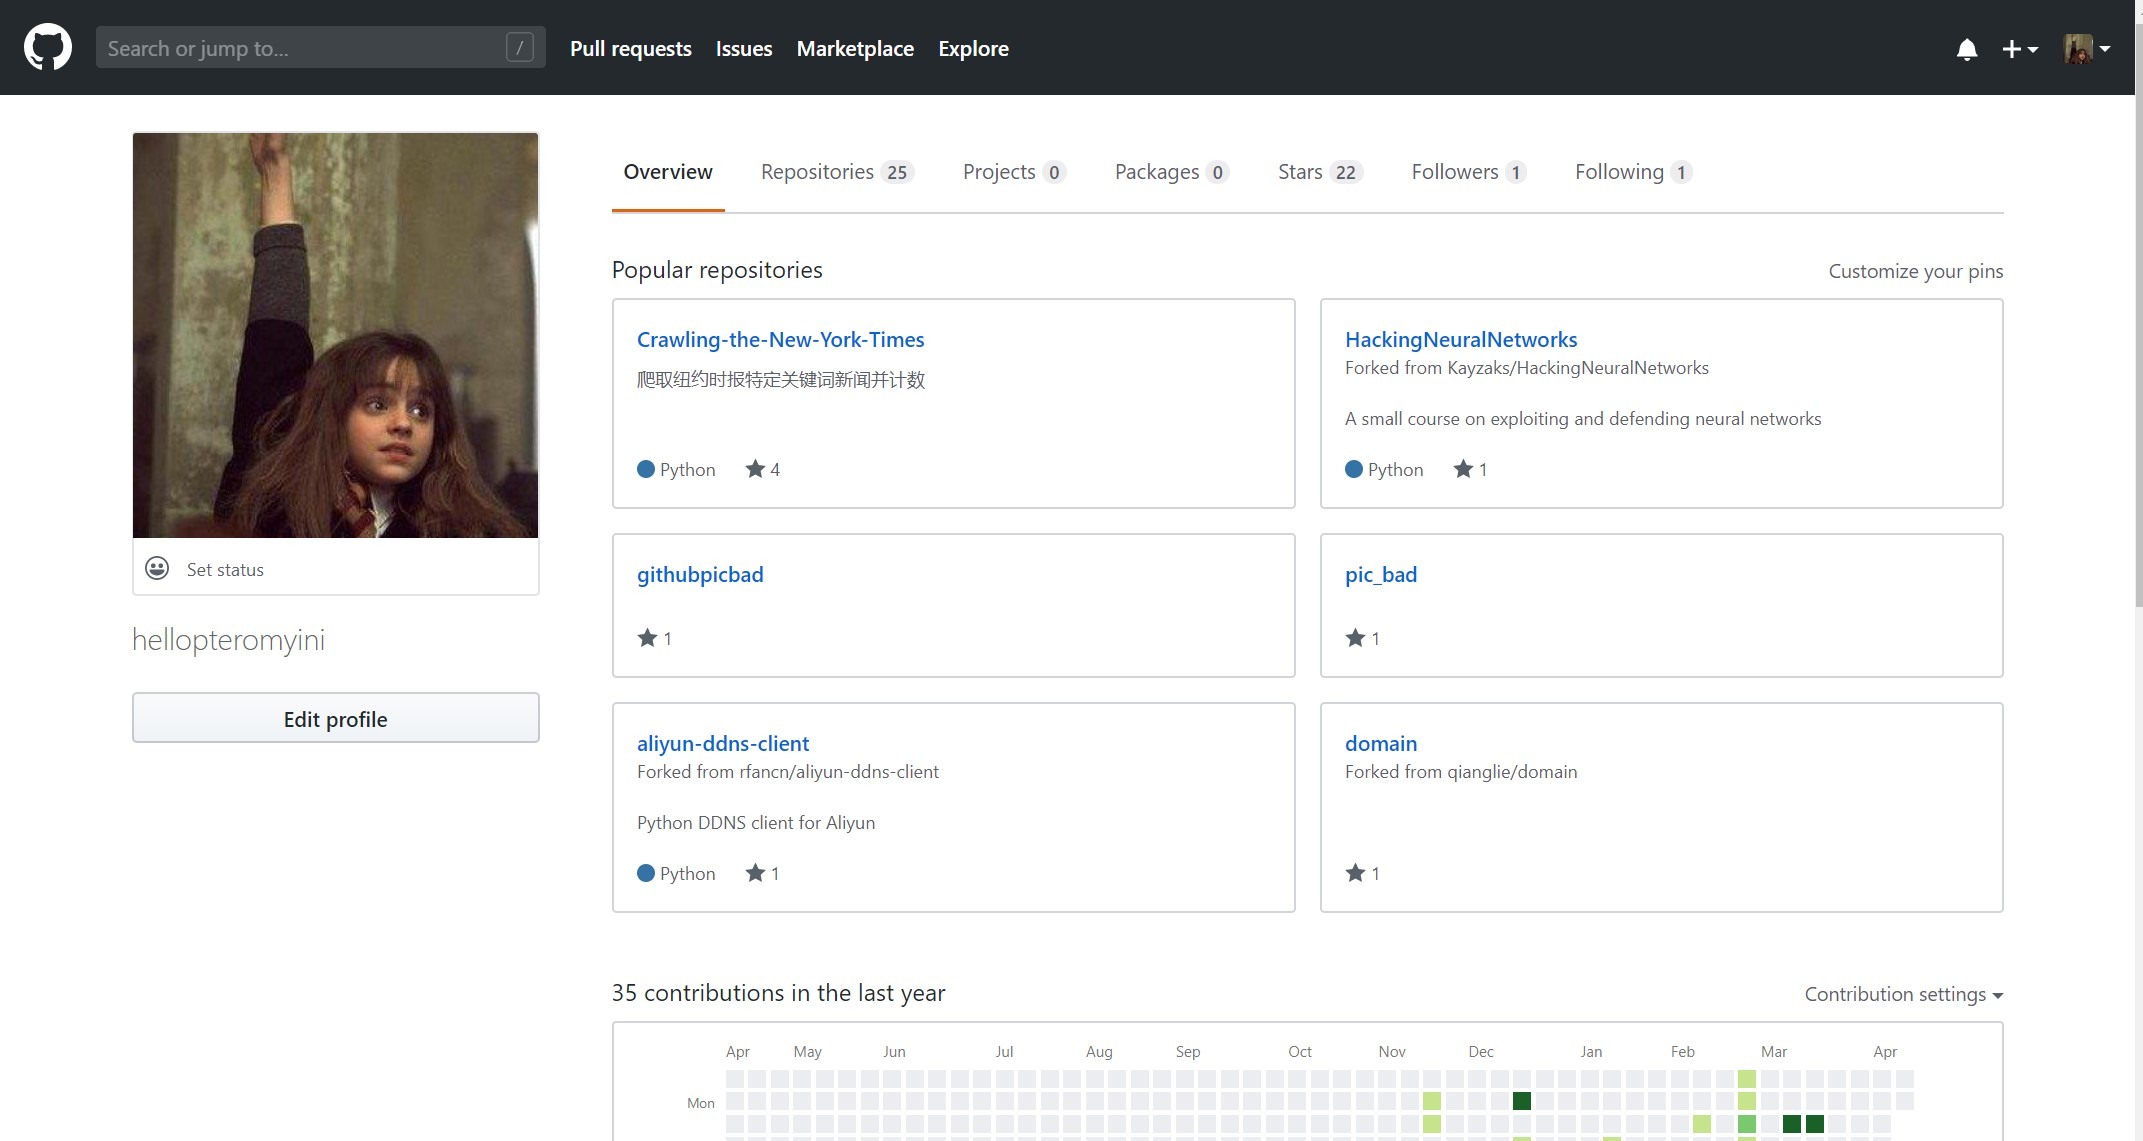
\includegraphics[width=12cm]{github}}
    \centerline{Github主页}
	\par 
	\item Bilibili主页
	\par
	\url{https://space.bilibili.com/58653603}
	\par
	\centerline{\includegraphics[width=12cm]{bilibili}}
	\centerline{Bilibili主页}
	\par
	\item 博客园博客
	\par
	\url{https://www.cnblogs.com/upcwsh/}
	\par
	\centerline{
\includegraphics[width=12cm]{cnblogs}}
	\centerline{博客园}	
	\par
	\item CSDN博客
	\par
	\url{https://blog.csdn.net/weixin_43797974}
	\par
	\centerline{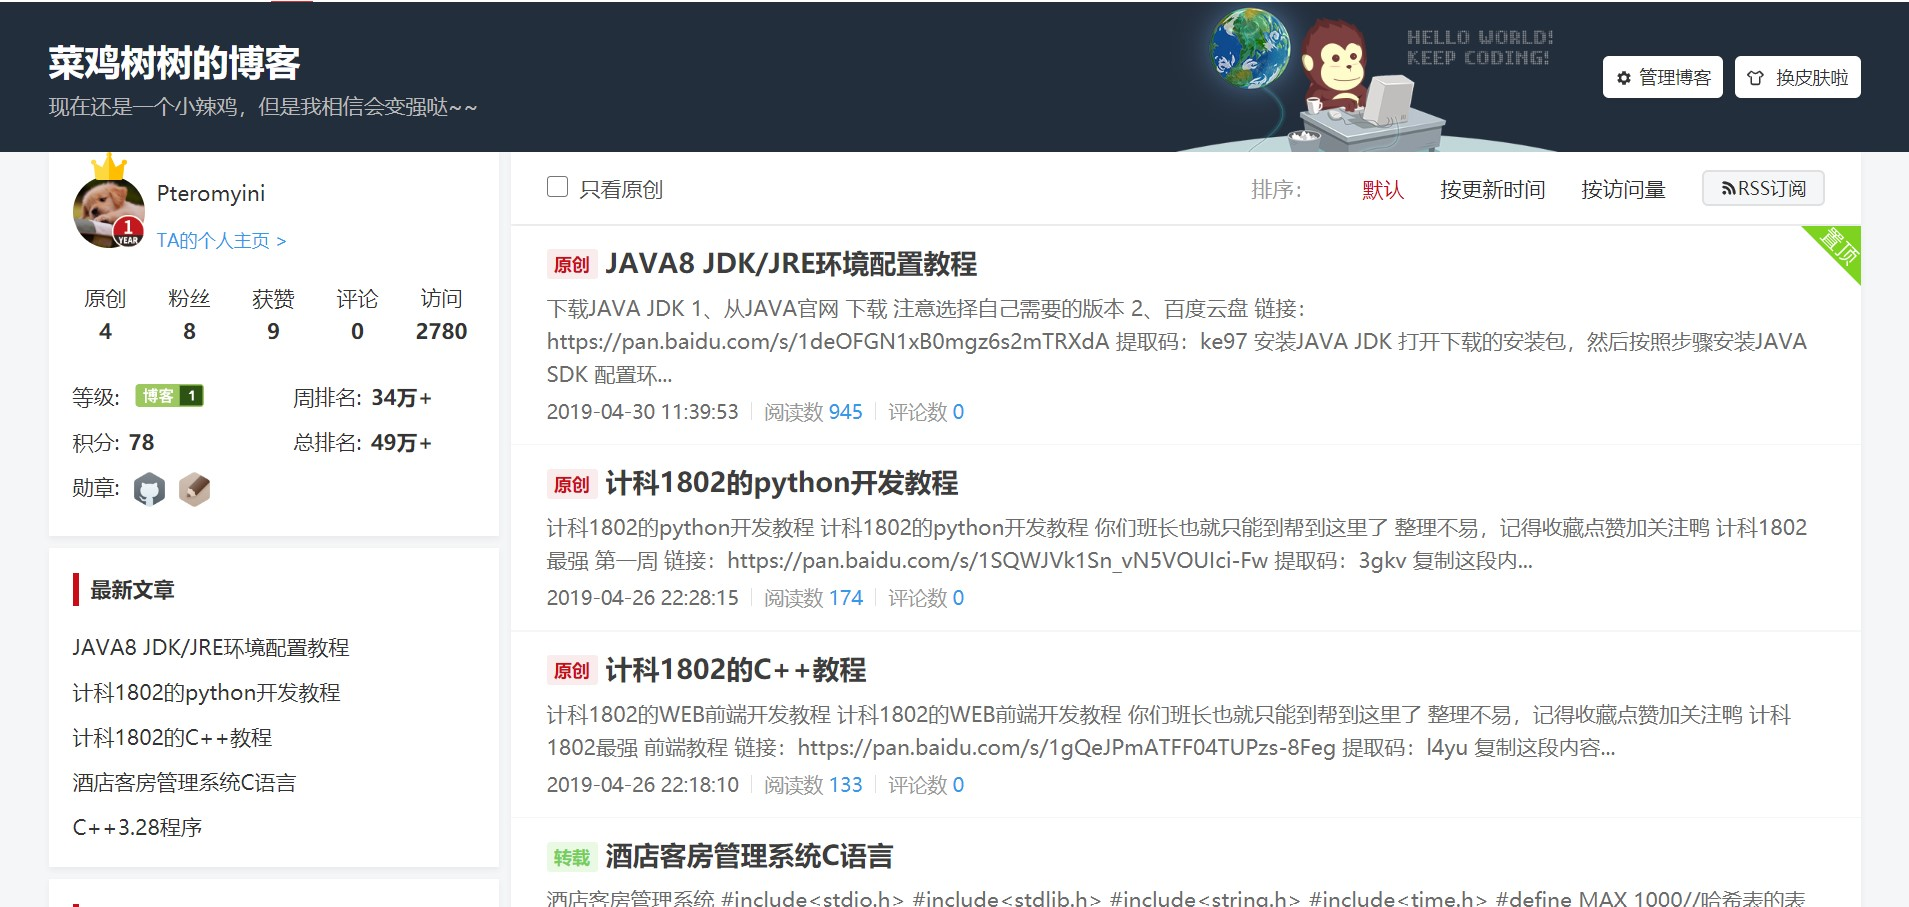
\includegraphics[width=12cm]{csdn}}
	\centerline{CSDN}	
	\par 
	\item 小木虫
	\par
	\url{http://muchong.com/bbs/space.php?uid=21828657}
	\par
	\centerline{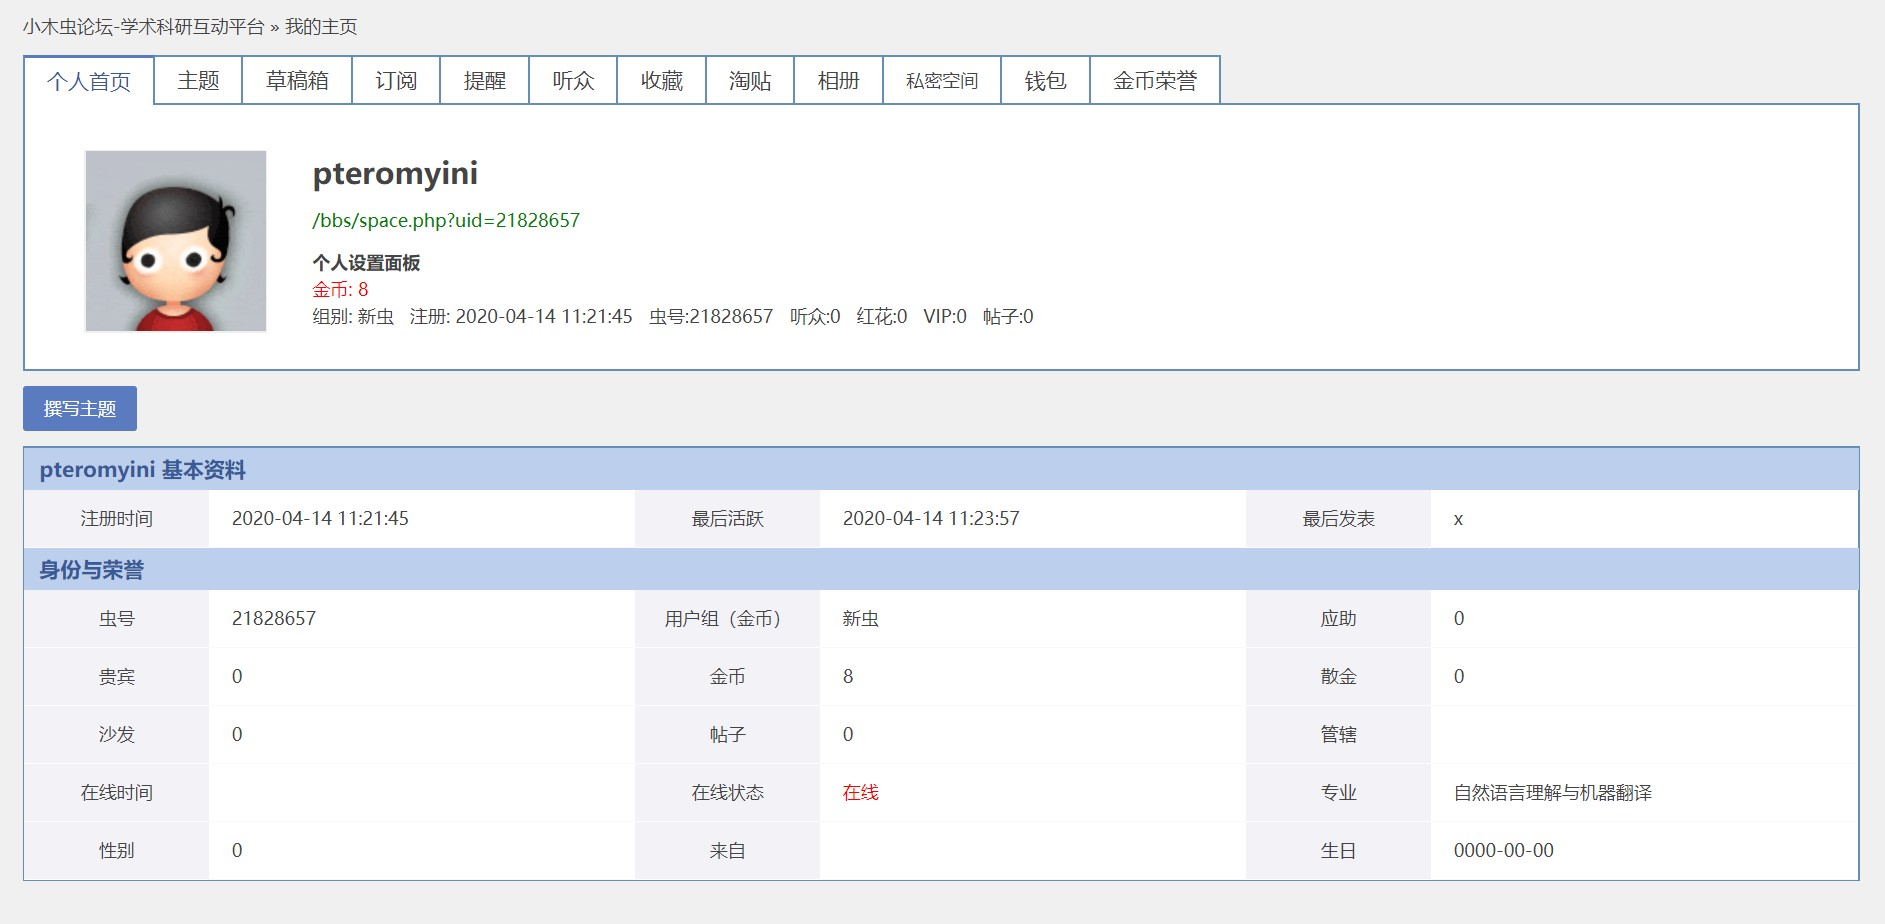
\includegraphics[width=12cm]{xiaomuchong}}
	\centerline{小木虫}	
	\par 
	\item 观察者网
	\par
	\centerline{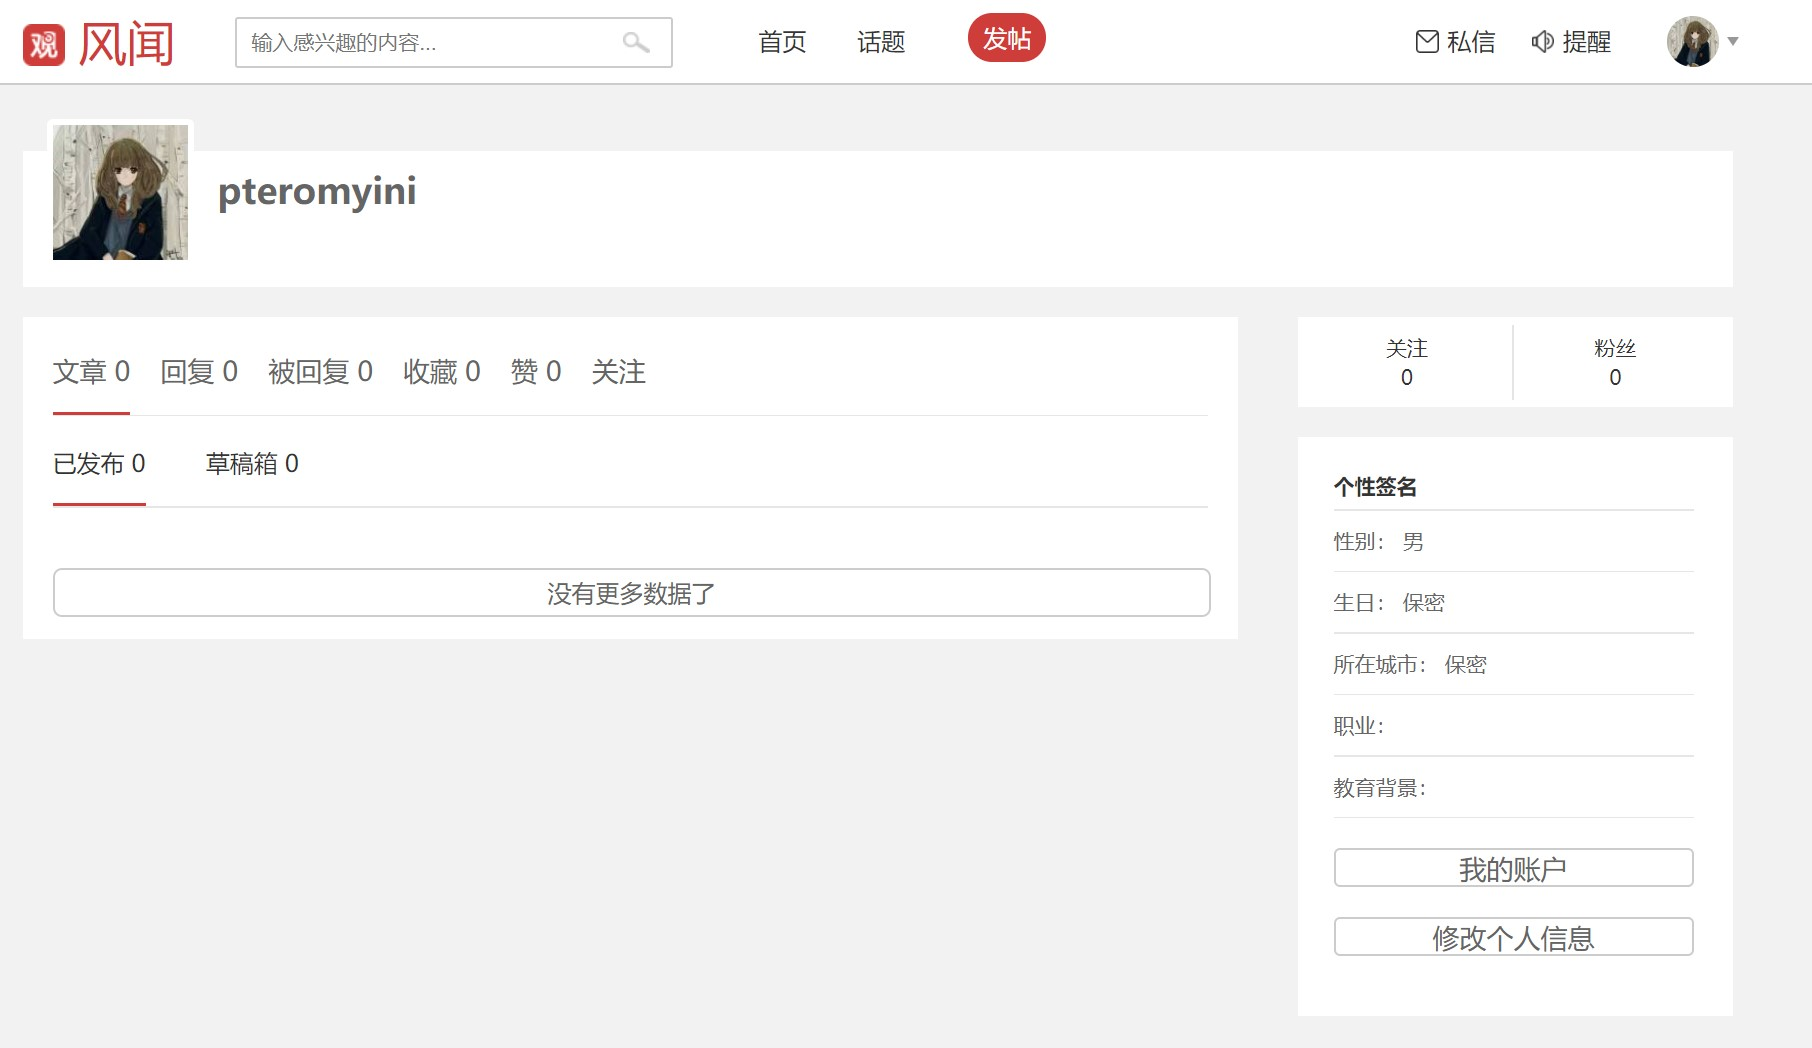
\includegraphics[width=12cm]{guanchazhe}}

\end{itemize}
\hspace*{\fill} \\
\bibliographystyle{plain}
\bibliography{references}
\end{document}
